\documentclass[twoside]{book}

% Packages required by doxygen
\usepackage{fixltx2e}
\usepackage{calc}
\usepackage{doxygen}
\usepackage{graphicx}
\usepackage[utf8]{inputenc}
\usepackage{makeidx}
\usepackage{multicol}
\usepackage{multirow}
\PassOptionsToPackage{warn}{textcomp}
\usepackage{textcomp}
\usepackage[nointegrals]{wasysym}
\usepackage[table]{xcolor}

% Font selection
\usepackage[T1]{fontenc}
\usepackage{mathptmx}
\usepackage[scaled=.90]{helvet}
\usepackage{courier}
\usepackage{amssymb}
\usepackage{sectsty}
\renewcommand{\familydefault}{\sfdefault}
\allsectionsfont{%
  \fontseries{bc}\selectfont%
  \color{darkgray}%
}
\renewcommand{\DoxyLabelFont}{%
  \fontseries{bc}\selectfont%
  \color{darkgray}%
}
\newcommand{\+}{\discretionary{\mbox{\scriptsize$\hookleftarrow$}}{}{}}

% Page & text layout
\usepackage{geometry}
\geometry{%
  a4paper,%
  top=2.5cm,%
  bottom=2.5cm,%
  left=2.5cm,%
  right=2.5cm%
}
\tolerance=750
\hfuzz=15pt
\hbadness=750
\setlength{\emergencystretch}{15pt}
\setlength{\parindent}{0cm}
\setlength{\parskip}{0.2cm}
\makeatletter
\renewcommand{\paragraph}{%
  \@startsection{paragraph}{4}{0ex}{-1.0ex}{1.0ex}{%
    \normalfont\normalsize\bfseries\SS@parafont%
  }%
}
\renewcommand{\subparagraph}{%
  \@startsection{subparagraph}{5}{0ex}{-1.0ex}{1.0ex}{%
    \normalfont\normalsize\bfseries\SS@subparafont%
  }%
}
\makeatother

% Headers & footers
\usepackage{fancyhdr}
\pagestyle{fancyplain}
\fancyhead[LE]{\fancyplain{}{\bfseries\thepage}}
\fancyhead[CE]{\fancyplain{}{}}
\fancyhead[RE]{\fancyplain{}{\bfseries\leftmark}}
\fancyhead[LO]{\fancyplain{}{\bfseries\rightmark}}
\fancyhead[CO]{\fancyplain{}{}}
\fancyhead[RO]{\fancyplain{}{\bfseries\thepage}}
\fancyfoot[LE]{\fancyplain{}{}}
\fancyfoot[CE]{\fancyplain{}{}}
\fancyfoot[RE]{\fancyplain{}{\bfseries\scriptsize Generated on Sun Nov 23 2014 23\+:20\+:27 for Queue by Doxygen }}
\fancyfoot[LO]{\fancyplain{}{\bfseries\scriptsize Generated on Sun Nov 23 2014 23\+:20\+:27 for Queue by Doxygen }}
\fancyfoot[CO]{\fancyplain{}{}}
\fancyfoot[RO]{\fancyplain{}{}}
\renewcommand{\footrulewidth}{0.4pt}
\renewcommand{\chaptermark}[1]{%
  \markboth{#1}{}%
}
\renewcommand{\sectionmark}[1]{%
  \markright{\thesection\ #1}%
}

% Indices & bibliography
\usepackage{natbib}
\usepackage[titles]{tocloft}
\setcounter{tocdepth}{3}
\setcounter{secnumdepth}{5}
\makeindex

% Hyperlinks (required, but should be loaded last)
\usepackage{ifpdf}
\ifpdf
  \usepackage[pdftex,pagebackref=true]{hyperref}
\else
  \usepackage[ps2pdf,pagebackref=true]{hyperref}
\fi
\hypersetup{%
  colorlinks=true,%
  linkcolor=blue,%
  citecolor=blue,%
  unicode%
}

% Custom commands
\newcommand{\clearemptydoublepage}{%
  \newpage{\pagestyle{empty}\cleardoublepage}%
}


%===== C O N T E N T S =====

\begin{document}

% Titlepage & ToC
\hypersetup{pageanchor=false,
             bookmarks=true,
             bookmarksnumbered=true,
             pdfencoding=unicode
            }
\pagenumbering{roman}
\begin{titlepage}
\vspace*{7cm}
\begin{center}%
{\Large Queue \\[1ex]\large 1.\+0 }\\
\vspace*{1cm}
{\large Generated by Doxygen 1.8.8}\\
\vspace*{0.5cm}
{\small Sun Nov 23 2014 23:20:27}\\
\end{center}
\end{titlepage}
\clearemptydoublepage
\tableofcontents
\clearemptydoublepage
\pagenumbering{arabic}
\hypersetup{pageanchor=true}

%--- Begin generated contents ---
\chapter{Hierarchical Index}
\section{Class Hierarchy}
This inheritance list is sorted roughly, but not completely, alphabetically\+:\begin{DoxyCompactList}
\item \contentsline{section}{Queue$<$ Data\+Type $>$}{\pageref{class_queue}}{}
\begin{DoxyCompactList}
\item \contentsline{section}{Queue\+Array$<$ Data\+Type $>$}{\pageref{class_queue_array}}{}
\item \contentsline{section}{Queue\+Linked$<$ Data\+Type $>$}{\pageref{class_queue_linked}}{}
\end{DoxyCompactList}
\end{DoxyCompactList}

\chapter{Class Index}
\section{Class List}
Here are the classes, structs, unions and interfaces with brief descriptions\+:\begin{DoxyCompactList}
\item\contentsline{section}{\hyperlink{class_expr_tree}{Expr\+Tree$<$ Data\+Type $>$} }{\pageref{class_expr_tree}}{}
\item\contentsline{section}{\hyperlink{class_expr_tree_1_1_expr_tree_node}{Expr\+Tree$<$ Data\+Type $>$\+::\+Expr\+Tree\+Node} }{\pageref{class_expr_tree_1_1_expr_tree_node}}{}
\end{DoxyCompactList}

\chapter{Class Documentation}
\hypertarget{class_queue}{\section{Queue$<$ Data\+Type $>$ Class Template Reference}
\label{class_queue}\index{Queue$<$ Data\+Type $>$@{Queue$<$ Data\+Type $>$}}
}
Inheritance diagram for Queue$<$ Data\+Type $>$\+:\begin{figure}[H]
\begin{center}
\leavevmode
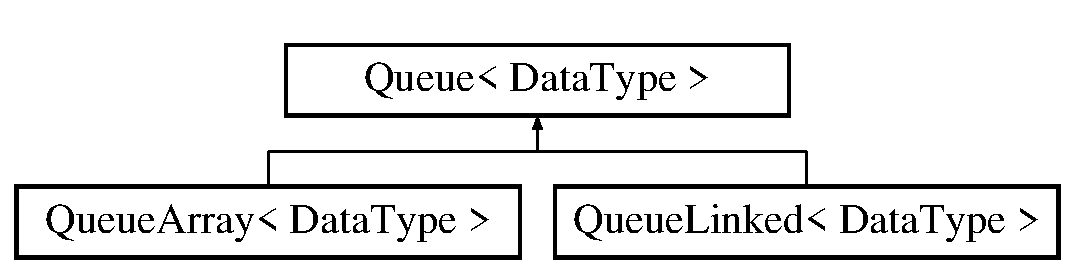
\includegraphics[height=2.000000cm]{class_queue}
\end{center}
\end{figure}
\subsection*{Public Member Functions}
\begin{DoxyCompactItemize}
\item 
\hypertarget{class_queue_a4e0052bab8c2fb742a16a77d73ec3d5a}{virtual void {\bfseries enqueue} (const Data\+Type \&new\+Data\+Item)=0  throw (logic\+\_\+error)}\label{class_queue_a4e0052bab8c2fb742a16a77d73ec3d5a}

\item 
\hypertarget{class_queue_afde1535196f515caba0aa5cfbe62d329}{virtual Data\+Type {\bfseries dequeue} ()=0  throw (logic\+\_\+error)}\label{class_queue_afde1535196f515caba0aa5cfbe62d329}

\item 
\hypertarget{class_queue_afba4d82c9a20859bb6397bd73c230cdd}{virtual void {\bfseries clear} ()=0}\label{class_queue_afba4d82c9a20859bb6397bd73c230cdd}

\item 
\hypertarget{class_queue_a1b8e1c0b8bb621de8d4f20c011176bd2}{virtual bool {\bfseries is\+Empty} () const =0}\label{class_queue_a1b8e1c0b8bb621de8d4f20c011176bd2}

\item 
\hypertarget{class_queue_ae64751e270709a705d49e6168e64ade8}{virtual bool {\bfseries is\+Full} () const =0}\label{class_queue_ae64751e270709a705d49e6168e64ade8}

\item 
\hypertarget{class_queue_a7db7279a763ca59f7fef354759beab17}{virtual void {\bfseries show\+Structure} () const =0}\label{class_queue_a7db7279a763ca59f7fef354759beab17}

\end{DoxyCompactItemize}
\subsection*{Static Public Attributes}
\begin{DoxyCompactItemize}
\item 
\hypertarget{class_queue_aaf3eed0540baaf6609b48910aacc7133}{static const int {\bfseries M\+A\+X\+\_\+\+Q\+U\+E\+U\+E\+\_\+\+S\+I\+Z\+E} = 8}\label{class_queue_aaf3eed0540baaf6609b48910aacc7133}

\end{DoxyCompactItemize}


The documentation for this class was generated from the following file\+:\begin{DoxyCompactItemize}
\item 
Queue.\+h\end{DoxyCompactItemize}

\hypertarget{class_queue_array}{\section{Queue\+Array$<$ Data\+Type $>$ Class Template Reference}
\label{class_queue_array}\index{Queue\+Array$<$ Data\+Type $>$@{Queue\+Array$<$ Data\+Type $>$}}
}
Inheritance diagram for Queue\+Array$<$ Data\+Type $>$\+:\begin{figure}[H]
\begin{center}
\leavevmode
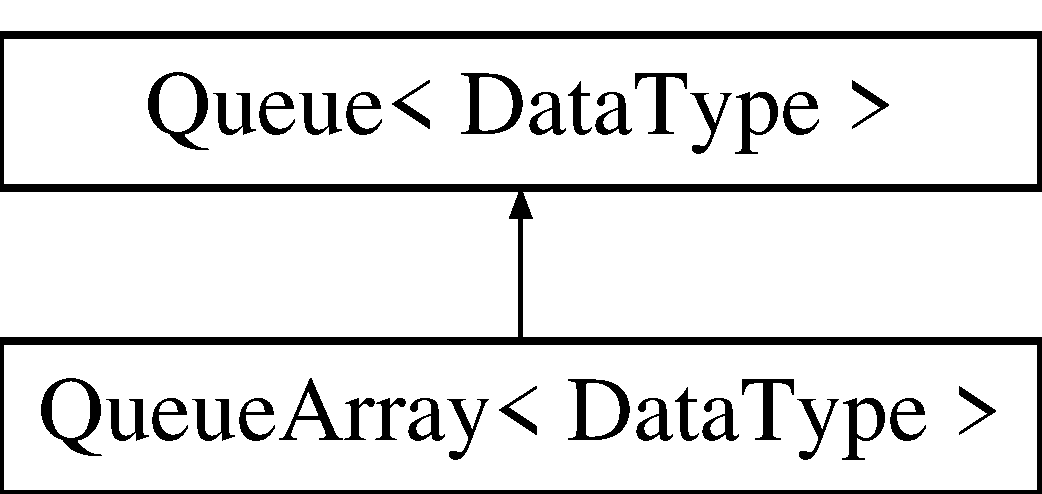
\includegraphics[height=2.000000cm]{class_queue_array}
\end{center}
\end{figure}
\subsection*{Public Member Functions}
\begin{DoxyCompactItemize}
\item 
\hypertarget{class_queue_array_a112114659f8c2590872426a2dee8e6cc}{{\bfseries Queue\+Array} (int max\+Number=\hyperlink{class_queue}{Queue}$<$ Data\+Type $>$\+::M\+A\+X\+\_\+\+Q\+U\+E\+U\+E\+\_\+\+S\+I\+Z\+E)}\label{class_queue_array_a112114659f8c2590872426a2dee8e6cc}

\item 
\hypertarget{class_queue_array_a08df206def55e930c9c561ee8bc93422}{{\bfseries Queue\+Array} (const \hyperlink{class_queue_array}{Queue\+Array} \&other)}\label{class_queue_array_a08df206def55e930c9c561ee8bc93422}

\item 
\hypertarget{class_queue_array_adaad55e5da06583cc786af90937a94c1}{\hyperlink{class_queue_array}{Queue\+Array} \& {\bfseries operator=} (const \hyperlink{class_queue_array}{Queue\+Array} \&other)}\label{class_queue_array_adaad55e5da06583cc786af90937a94c1}

\item 
\hypertarget{class_queue_array_a15e0632c580858c396d3aac1265fecd7}{void {\bfseries enqueue} (const Data\+Type \&new\+Data\+Item)  throw (logic\+\_\+error)}\label{class_queue_array_a15e0632c580858c396d3aac1265fecd7}

\item 
\hypertarget{class_queue_array_a34d386d2323aa80b7b441d4436153a89}{Data\+Type {\bfseries dequeue} ()  throw (logic\+\_\+error)}\label{class_queue_array_a34d386d2323aa80b7b441d4436153a89}

\item 
\hypertarget{class_queue_array_a154afbf4084cb08e3a134f2f6a33df6c}{void {\bfseries clear} ()}\label{class_queue_array_a154afbf4084cb08e3a134f2f6a33df6c}

\item 
\hypertarget{class_queue_array_ae1298c7e16e1053b628a019e71db4320}{bool {\bfseries is\+Empty} () const }\label{class_queue_array_ae1298c7e16e1053b628a019e71db4320}

\item 
\hypertarget{class_queue_array_a7233d591dd81e9e3d3f6e4ad5631c81c}{bool {\bfseries is\+Full} () const }\label{class_queue_array_a7233d591dd81e9e3d3f6e4ad5631c81c}

\item 
\hypertarget{class_queue_array_add18fcb931a244d56040a1f0a0c24a8f}{void {\bfseries put\+Front} (const Data\+Type \&new\+Data\+Item)  throw (logic\+\_\+error)}\label{class_queue_array_add18fcb931a244d56040a1f0a0c24a8f}

\item 
\hypertarget{class_queue_array_a8bebf91214e116f74d4482bf9babee2d}{Data\+Type {\bfseries get\+Rear} ()  throw (logic\+\_\+error)}\label{class_queue_array_a8bebf91214e116f74d4482bf9babee2d}

\item 
\hypertarget{class_queue_array_a1d1bf41a4ca23c30f53296a0e0c5bf33}{int {\bfseries get\+Length} () const }\label{class_queue_array_a1d1bf41a4ca23c30f53296a0e0c5bf33}

\item 
\hypertarget{class_queue_array_adde651b7fd7865dc4f281e21c7f1a6c3}{void {\bfseries show\+Structure} () const }\label{class_queue_array_adde651b7fd7865dc4f281e21c7f1a6c3}

\end{DoxyCompactItemize}
\subsection*{Additional Inherited Members}


The documentation for this class was generated from the following file\+:\begin{DoxyCompactItemize}
\item 
Queue\+Array.\+h\end{DoxyCompactItemize}

\hypertarget{class_queue_linked}{\section{Queue\+Linked$<$ Data\+Type $>$ Class Template Reference}
\label{class_queue_linked}\index{Queue\+Linked$<$ Data\+Type $>$@{Queue\+Linked$<$ Data\+Type $>$}}
}
Inheritance diagram for Queue\+Linked$<$ Data\+Type $>$\+:\begin{figure}[H]
\begin{center}
\leavevmode
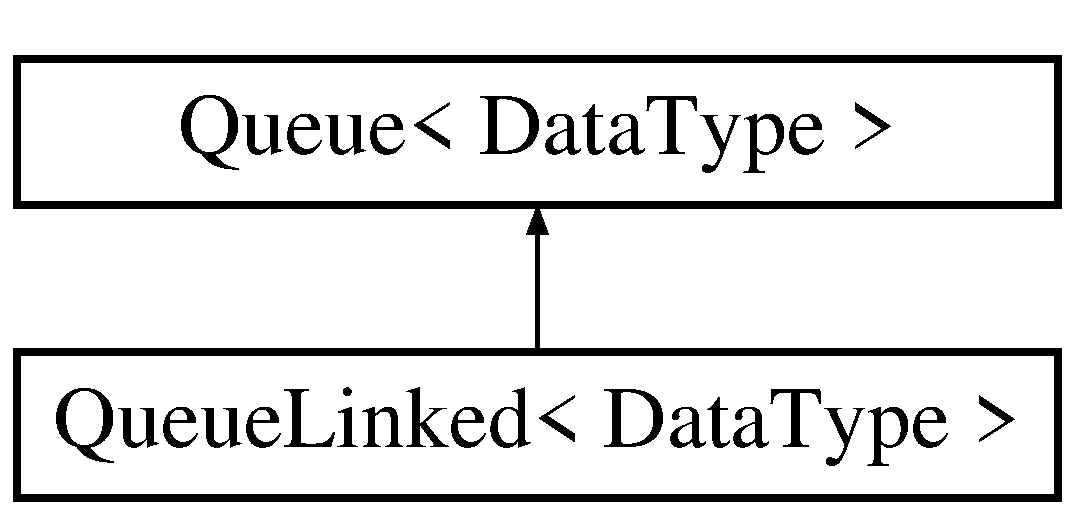
\includegraphics[height=2.000000cm]{class_queue_linked}
\end{center}
\end{figure}
\subsection*{Public Member Functions}
\begin{DoxyCompactItemize}
\item 
\hyperlink{class_queue_linked_ad356fca32ffd90c78d35d3eb5d84504b}{Queue\+Linked} (int max\+Number=\hyperlink{class_queue}{Queue}$<$ Data\+Type $>$\+::M\+A\+X\+\_\+\+Q\+U\+E\+U\+E\+\_\+\+S\+I\+Z\+E)
\item 
\hyperlink{class_queue_linked_ad8749850191f8a4165c8e3a3a266bada}{Queue\+Linked} (const \hyperlink{class_queue_linked}{Queue\+Linked} \&other)
\item 
\hypertarget{class_queue_linked_acec147d4de2139d2b6fd511bca6d6299}{\hyperlink{class_queue_linked}{Queue\+Linked} \& \hyperlink{class_queue_linked_acec147d4de2139d2b6fd511bca6d6299}{operator=} (const \hyperlink{class_queue_linked}{Queue\+Linked} \&other)}\label{class_queue_linked_acec147d4de2139d2b6fd511bca6d6299}

\begin{DoxyCompactList}\small\item\em Assignment operator overloaded. \end{DoxyCompactList}\item 
\hyperlink{class_queue_linked_aed85fa73c60384a3d0c676c0ebbbca19}{$\sim$\+Queue\+Linked} ()
\item 
void \hyperlink{class_queue_linked_a7196448729d053f85f255674c7a57a02}{enqueue} (const Data\+Type \&new\+Data\+Item)  throw (logic\+\_\+error)
\item 
Data\+Type \hyperlink{class_queue_linked_ac0656892f605af3b952c71706d3af55d}{dequeue} ()  throw (logic\+\_\+error)
\item 
void \hyperlink{class_queue_linked_a32c66945765e5d42bbb988b1cdf43886}{clear} ()
\item 
bool \hyperlink{class_queue_linked_a425b83383323217c924a41a0226f7022}{is\+Empty} () const 
\item 
bool \hyperlink{class_queue_linked_a3de199675ee629f9d20c48d0e2b65f71}{is\+Full} () const 
\item 
void \hyperlink{class_queue_linked_a838a51b8023f9cf3a5a24abb67ae1ee4}{put\+Front} (const Data\+Type \&new\+Data\+Item)  throw (logic\+\_\+error)
\item 
Data\+Type \hyperlink{class_queue_linked_a2934f746096e31b9728de11f42bdc3cd}{get\+Rear} ()  throw (logic\+\_\+error)
\item 
int \hyperlink{class_queue_linked_ab2d7fc0a927f3fe1e2ac44cc042bb961}{get\+Length} () const 
\item 
\hypertarget{class_queue_linked_a57d5dd5336545ddc7d1b22cee40fb017}{void {\bfseries show\+Structure} () const }\label{class_queue_linked_a57d5dd5336545ddc7d1b22cee40fb017}

\end{DoxyCompactItemize}
\subsection*{Additional Inherited Members}


\subsection{Constructor \& Destructor Documentation}
\hypertarget{class_queue_linked_ad356fca32ffd90c78d35d3eb5d84504b}{\index{Queue\+Linked@{Queue\+Linked}!Queue\+Linked@{Queue\+Linked}}
\index{Queue\+Linked@{Queue\+Linked}!Queue\+Linked@{Queue\+Linked}}
\subsubsection[{Queue\+Linked}]{\setlength{\rightskip}{0pt plus 5cm}template$<$typename Data\+Type $>$ {\bf Queue\+Linked}$<$ Data\+Type $>$\+::{\bf Queue\+Linked} (
\begin{DoxyParamCaption}
\item[{int}]{max\+Number = {\ttfamily {\bf Queue}$<$DataType$>$\+:\+:MAX\+\_\+QUEUE\+\_\+SIZE}}
\end{DoxyParamCaption}
)}}\label{class_queue_linked_ad356fca32ffd90c78d35d3eb5d84504b}
Default Constructor, sets pointers to N\+U\+L\+L input parameter is irrelevant since we have no max size \hypertarget{class_queue_linked_ad8749850191f8a4165c8e3a3a266bada}{\index{Queue\+Linked@{Queue\+Linked}!Queue\+Linked@{Queue\+Linked}}
\index{Queue\+Linked@{Queue\+Linked}!Queue\+Linked@{Queue\+Linked}}
\subsubsection[{Queue\+Linked}]{\setlength{\rightskip}{0pt plus 5cm}template$<$typename Data\+Type $>$ {\bf Queue\+Linked}$<$ Data\+Type $>$\+::{\bf Queue\+Linked} (
\begin{DoxyParamCaption}
\item[{const {\bf Queue\+Linked}$<$ Data\+Type $>$ \&}]{other}
\end{DoxyParamCaption}
)}}\label{class_queue_linked_ad8749850191f8a4165c8e3a3a266bada}
Copy Constructor copies the input parameter of another queue if it is empty just set pointers to N\+U\+L\+L otherwise copy \hypertarget{class_queue_linked_aed85fa73c60384a3d0c676c0ebbbca19}{\index{Queue\+Linked@{Queue\+Linked}!````~Queue\+Linked@{$\sim$\+Queue\+Linked}}
\index{````~Queue\+Linked@{$\sim$\+Queue\+Linked}!Queue\+Linked@{Queue\+Linked}}
\subsubsection[{$\sim$\+Queue\+Linked}]{\setlength{\rightskip}{0pt plus 5cm}template$<$typename Data\+Type $>$ {\bf Queue\+Linked}$<$ Data\+Type $>$\+::$\sim${\bf Queue\+Linked} (
\begin{DoxyParamCaption}
{}
\end{DoxyParamCaption}
)}}\label{class_queue_linked_aed85fa73c60384a3d0c676c0ebbbca19}
Deconstructor clears all memory 

\subsection{Member Function Documentation}
\hypertarget{class_queue_linked_a32c66945765e5d42bbb988b1cdf43886}{\index{Queue\+Linked@{Queue\+Linked}!clear@{clear}}
\index{clear@{clear}!Queue\+Linked@{Queue\+Linked}}
\subsubsection[{clear}]{\setlength{\rightskip}{0pt plus 5cm}template$<$typename Data\+Type $>$ void {\bf Queue\+Linked}$<$ Data\+Type $>$\+::clear (
\begin{DoxyParamCaption}
{}
\end{DoxyParamCaption}
)\hspace{0.3cm}{\ttfamily [virtual]}}}\label{class_queue_linked_a32c66945765e5d42bbb988b1cdf43886}
clear deletes all allocated memory for the queue nodes 

Implements \hyperlink{class_queue}{Queue$<$ Data\+Type $>$}.

\hypertarget{class_queue_linked_ac0656892f605af3b952c71706d3af55d}{\index{Queue\+Linked@{Queue\+Linked}!dequeue@{dequeue}}
\index{dequeue@{dequeue}!Queue\+Linked@{Queue\+Linked}}
\subsubsection[{dequeue}]{\setlength{\rightskip}{0pt plus 5cm}template$<$typename Data\+Type $>$ Data\+Type {\bf Queue\+Linked}$<$ Data\+Type $>$\+::dequeue (
\begin{DoxyParamCaption}
{}
\end{DoxyParamCaption}
) throw  logic\+\_\+error) \hspace{0.3cm}{\ttfamily [virtual]}}}\label{class_queue_linked_ac0656892f605af3b952c71706d3af55d}
dequeue takes the front data 

Implements \hyperlink{class_queue}{Queue$<$ Data\+Type $>$}.

\hypertarget{class_queue_linked_a7196448729d053f85f255674c7a57a02}{\index{Queue\+Linked@{Queue\+Linked}!enqueue@{enqueue}}
\index{enqueue@{enqueue}!Queue\+Linked@{Queue\+Linked}}
\subsubsection[{enqueue}]{\setlength{\rightskip}{0pt plus 5cm}template$<$typename Data\+Type $>$ void {\bf Queue\+Linked}$<$ Data\+Type $>$\+::enqueue (
\begin{DoxyParamCaption}
\item[{const Data\+Type \&}]{new\+Data\+Item}
\end{DoxyParamCaption}
) throw  logic\+\_\+error) \hspace{0.3cm}{\ttfamily [virtual]}}}\label{class_queue_linked_a7196448729d053f85f255674c7a57a02}
Enqueue adds new data to queue create new node

if the current is empty make first (just realized this could have been coded better, too late to fix/test) 

Implements \hyperlink{class_queue}{Queue$<$ Data\+Type $>$}.

\hypertarget{class_queue_linked_ab2d7fc0a927f3fe1e2ac44cc042bb961}{\index{Queue\+Linked@{Queue\+Linked}!get\+Length@{get\+Length}}
\index{get\+Length@{get\+Length}!Queue\+Linked@{Queue\+Linked}}
\subsubsection[{get\+Length}]{\setlength{\rightskip}{0pt plus 5cm}template$<$typename Data\+Type $>$ int {\bf Queue\+Linked}$<$ Data\+Type $>$\+::get\+Length (
\begin{DoxyParamCaption}
{}
\end{DoxyParamCaption}
) const}}\label{class_queue_linked_ab2d7fc0a927f3fe1e2ac44cc042bb961}
getlength returns the length of the queue \hypertarget{class_queue_linked_a2934f746096e31b9728de11f42bdc3cd}{\index{Queue\+Linked@{Queue\+Linked}!get\+Rear@{get\+Rear}}
\index{get\+Rear@{get\+Rear}!Queue\+Linked@{Queue\+Linked}}
\subsubsection[{get\+Rear}]{\setlength{\rightskip}{0pt plus 5cm}template$<$typename Data\+Type $>$ Data\+Type {\bf Queue\+Linked}$<$ Data\+Type $>$\+::get\+Rear (
\begin{DoxyParamCaption}
{}
\end{DoxyParamCaption}
) throw  logic\+\_\+error) }}\label{class_queue_linked_a2934f746096e31b9728de11f42bdc3cd}
getrear grabs the last data item in the queue check for empty

if there is only one item

save the back

go to prior

delete the last

set the next of the new back to null \hypertarget{class_queue_linked_a425b83383323217c924a41a0226f7022}{\index{Queue\+Linked@{Queue\+Linked}!is\+Empty@{is\+Empty}}
\index{is\+Empty@{is\+Empty}!Queue\+Linked@{Queue\+Linked}}
\subsubsection[{is\+Empty}]{\setlength{\rightskip}{0pt plus 5cm}template$<$typename Data\+Type $>$ bool {\bf Queue\+Linked}$<$ Data\+Type $>$\+::is\+Empty (
\begin{DoxyParamCaption}
{}
\end{DoxyParamCaption}
) const\hspace{0.3cm}{\ttfamily [virtual]}}}\label{class_queue_linked_a425b83383323217c924a41a0226f7022}
is\+Empty checks to see if the queue has any data 

Implements \hyperlink{class_queue}{Queue$<$ Data\+Type $>$}.

\hypertarget{class_queue_linked_a3de199675ee629f9d20c48d0e2b65f71}{\index{Queue\+Linked@{Queue\+Linked}!is\+Full@{is\+Full}}
\index{is\+Full@{is\+Full}!Queue\+Linked@{Queue\+Linked}}
\subsubsection[{is\+Full}]{\setlength{\rightskip}{0pt plus 5cm}template$<$typename Data\+Type $>$ bool {\bf Queue\+Linked}$<$ Data\+Type $>$\+::is\+Full (
\begin{DoxyParamCaption}
{}
\end{DoxyParamCaption}
) const\hspace{0.3cm}{\ttfamily [virtual]}}}\label{class_queue_linked_a3de199675ee629f9d20c48d0e2b65f71}
if\+Full irrelevant because always false 

Implements \hyperlink{class_queue}{Queue$<$ Data\+Type $>$}.

\hypertarget{class_queue_linked_a838a51b8023f9cf3a5a24abb67ae1ee4}{\index{Queue\+Linked@{Queue\+Linked}!put\+Front@{put\+Front}}
\index{put\+Front@{put\+Front}!Queue\+Linked@{Queue\+Linked}}
\subsubsection[{put\+Front}]{\setlength{\rightskip}{0pt plus 5cm}template$<$typename Data\+Type $>$ void {\bf Queue\+Linked}$<$ Data\+Type $>$\+::put\+Front (
\begin{DoxyParamCaption}
\item[{const Data\+Type \&}]{new\+Data\+Item}
\end{DoxyParamCaption}
) throw  logic\+\_\+error) }}\label{class_queue_linked_a838a51b8023f9cf3a5a24abb67ae1ee4}
putfront will add new data to the queue but differently than enqueue, will put the newest data up front 

The documentation for this class was generated from the following files\+:\begin{DoxyCompactItemize}
\item 
Queue\+Linked.\+h\item 
Queue\+Linked.\+cpp\end{DoxyCompactItemize}

%--- End generated contents ---

% Index
\newpage
\phantomsection
\addcontentsline{toc}{chapter}{Index}
\printindex

\end{document}
